%%%%%%%%%%%%%%%%%%%%%%%%%%%%%%%%%%%%%%%%%%%%%%%%%%%%%%%%%%%%%%%%%%%%%%%%
% Plantilla TFG/TFM
% Escuela Politécnica Superior de la Universidad de Alicante
% Realizado por: Jose Manuel Requena Plens
% Contacto: info@jmrplens.com / Telegram:@jmrplens
%%%%%%%%%%%%%%%%%%%%%%%%%%%%%%%%%%%%%%%%%%%%%%%%%%%%%%%%%%%%%%%%%%%%%%%%

\chapter{Desarrollo}
\label{desarrollo}

Como he comentado en el apartado de metodología, el desarrollo del \gls{tfg} se divide en iteraciones, de las cuales ha habido un total de 9, y en los siguientes apartados expondré cuál es el trabajo que se ha desarrollado en el transcurso de las mismas.
Por lo tanto, este apartado será el más extendido del \gls{tfg}, ya que en él explico detalladamente cuál es el trabajo que he ido haciendo, ordenado en el tiempo, y dividido en los tempos que me he reunido con mi tutor.

\section{Primera iteración: desarrollo del motor}
El \textbf{7 de julio de 2020} nos citamos por la herramienta Google Meet, y hablamos sobre cuál era mi objetivo con este \gls{tfg}, lo definimos y presentamos la propuesta. Además, como no tenía conocimientos sobre motores de videojuegos, me sugirió empezar viendo su curso para desarrollar un motor en C/C++. No concertamos una segunda cita ya que empezaba la época de verano, y quedamos en que cuando comenzara el curso y hubiera desarrollado mi motor volvería a ponerme en contacto con él.

\subsection{Script de construcción del proyecto}
Lo primero que hice fue, antes de ponerme a programar el motor, crear el archivo Makefile, este es el fichero que la herramienta Make ya mencionada en el apartado \ref{herramientas} de herramientas, utiliza como Build Script. De esta forma no tendría que compilar todos los archivos uno a uno. Y además, separando las librerías del resto del código, así no tendrían que ser re-compiladas cada vez que necesite crear un ejecutable, ya que este es un proceso que tarda unos segundos pero se repite muchas veces, por lo que estos segundos ahorrados a lo largo del desarrollo podrían llegar a ser muchos minutos, incluso horas, de espera ahorrados.

Como no voy a explicar todo el archivo línea por línea, lo haré con las partes más importantes del mismo. 
\begin{itemize}
	\item La macro \textbf{COMPILE}, recibe cinco parámetros. Es usada para compilar todos los objetos antes de ser enlazados. Recibe los siguientes parámetros:
	\begin{enumerate}
		\item Compilador a usar (gcc, g++, clang++, etc.)
		\item Nombre del objeto que se genera
		\item Archivos de código fuente
		\item Dependencias
		\item Flags para el compilador
	\end{enumerate}
	\begin{lstlisting}[style=C, caption={Macro Compile del Makefile},label=macro-compile]
		define COMPILE
		$(2) : $(3) $(4)
			$(1) -c -o $(2) $(3) $(5)
		endef
	\end{lstlisting}
	\item La instrucción \textbf{\$(APP)} o \textbf{game}, que es el nombre del ejecutable final. 
	\begin{itemize} 
		\item Depende de todos los objetos. 
		\item Enlaza todos los objetos y librerías, y genera el ejecutable
	\end{itemize}
	\begin{lstlisting}[style=C, caption={Enlazado de los objetos y las librerías para generar el ejecutable.},label=library-linking]
	$(APP) : $(OBJSUBDIRS) $(ALLOBJ)
		$(CC) -o $(APP) $(ALLOBJ) $(LIB) $(CCFLAGS)
	\end{lstlisting}
	\item La instrucción \textbf{clean}, que elimina los objetos para re-compilarlos desde cero.
	\item La instrucción \textbf{libs} y \textbf{libs-clean}, que compila y elimina pero con las librerías.
\end{itemize}
Dentro de la carpeta lib tenemos otro Makefile que sirve para compilar las librerias, las cuales tienen su propio Makefile también, muy parecido al ya mencionado.

\subsection{Motor de videojuego}
Comenzamos el desarrollo del videojuego creando el motor, pues sin él, no se puede avanzar con los otros puntos. Se trata de un motor \gls{ecs}\footnote{Conocido en español como Sistema de Entidades y Componentes. Es un patrón de desarrollo para motores de videojuegos.} el cual se basa en que las entidades son manejadas por el motor, mientras que los componentes (como físicas, renderizado, colisiones, etc.) son añadidos desde el juego. Pero el motor es el que se encarga de añadir los componentes a las entidades o destruirlos. Y los sistemas son los encargados de actualizar el estado de los componentes.

Para que el motor se comporte de manera eficiente con la caché, todos los componentes de un mismo tipo se almacenan seguidos en memoria, para que así, cada sistema del juego pida un solo tipo de componente de todas las entidades del juego. Ya que se ha demostrado que leer un dato de la caché es, de media, 200 veces más rápido que leerlo de la RAM, y cuando el programa pide un dato, no solo se carga ese dato pedido, sino un stream de datos. Además, cabe mencionar que la caché lee de la memoria RAM por líneas, nunca lee menos del tamaño de una linea, como se puede apreciar en el ejemplo de la figura \ref{Memoria RAM y CPU}, con una linea de caché de 64 bytes de tamaño.
\begin{figure}[H]
	\centering
	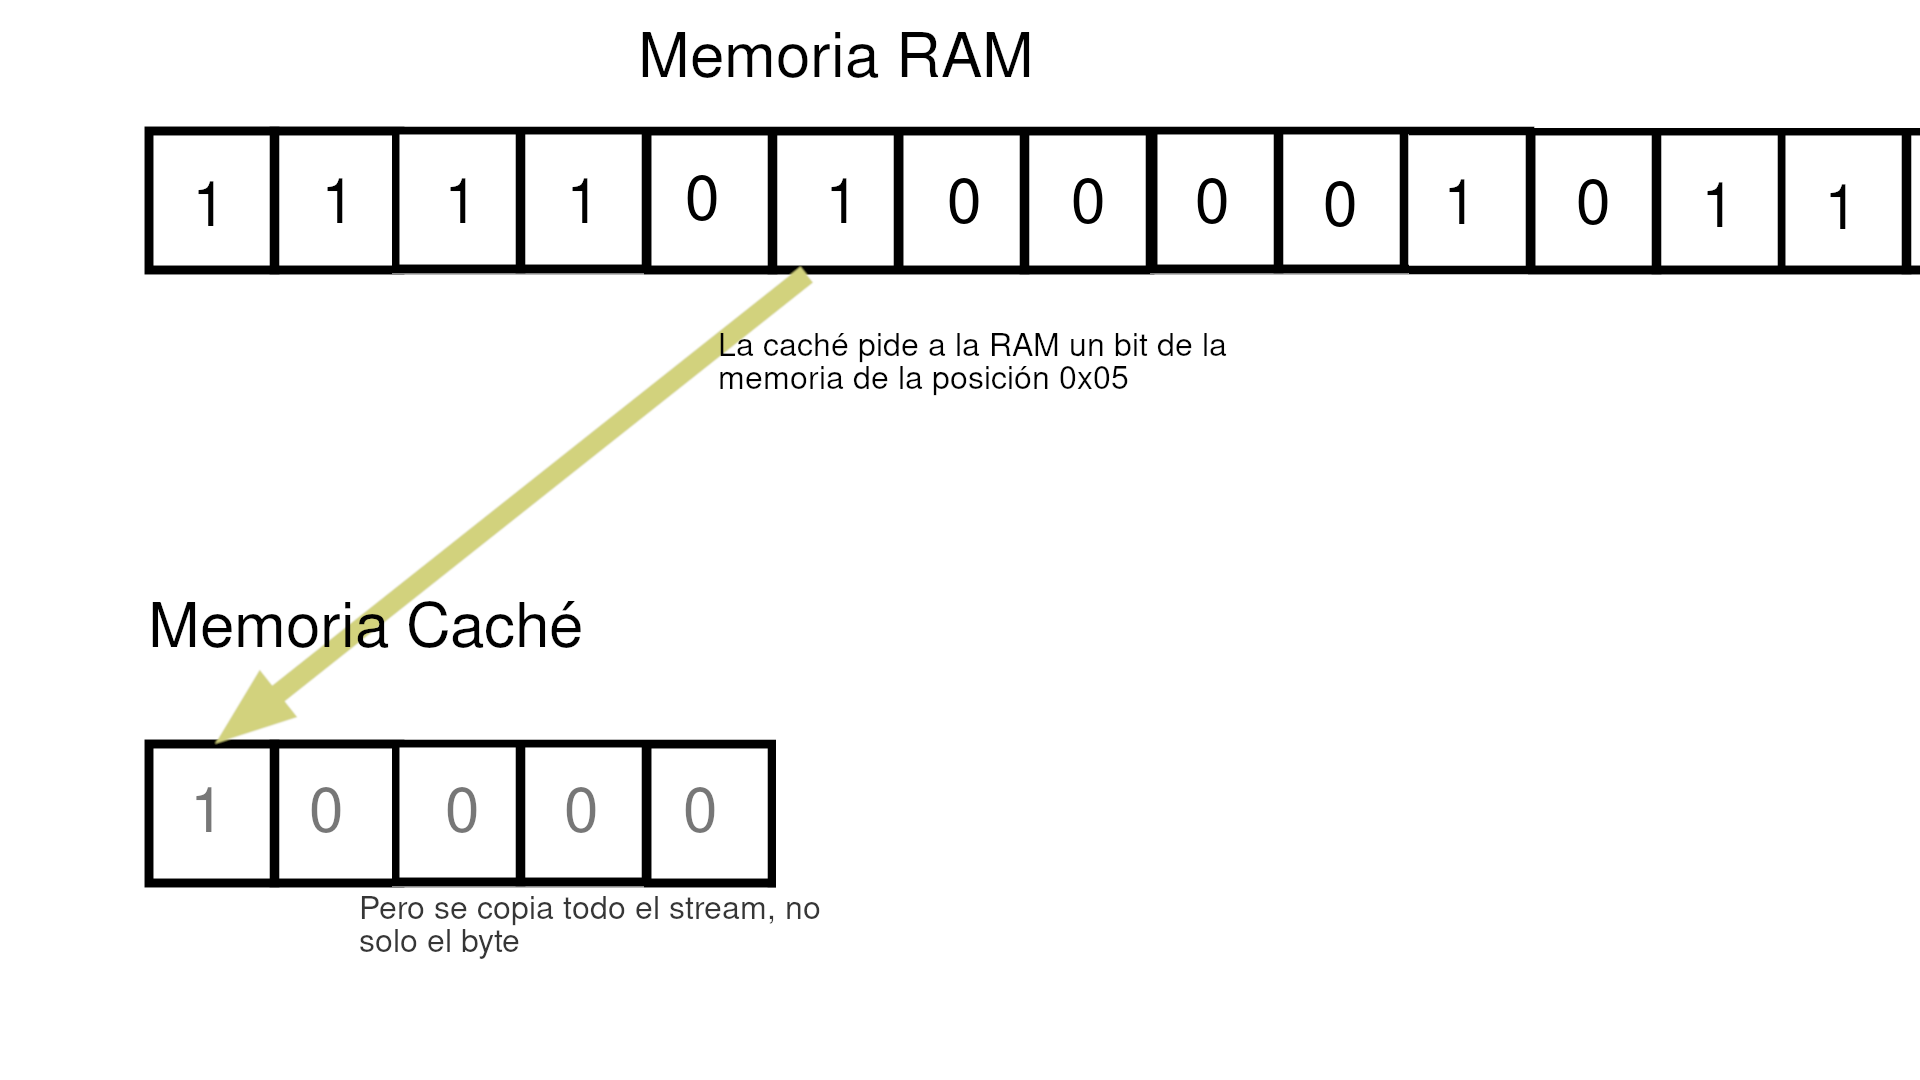
\includegraphics[width=15cm]{archivos/imagenes/comportamiento-memoria-cpu-ram.png}
	\caption{Comportamiento de la memoria CPU cuando lee de la RAM.}
	\label{Memoria RAM y CPU}
\end{figure}

¿Cómo se pueden alinear los datos en memoria según su tipo? La implementación ha sido usando la librería unordered\_map de C++, con la cual podremos usar un mapa, es decir, una estructura de datos en la que uno es el identificador (el tipo de dato, en este caso), y otro es el valor almacenado (un vector de componentes, en este caso).  Esto trae un problema consigo, porque el ``tipo de dato'' no es un tipo básico en C++, esto explicaré más adelante cómo lo solucionaremos. 

Cada sistema es encargado de un tipo de componente, para así poder recorrer la memoria de forma lineal como ya hemos mencionado antes (el sistema de físicas recorre todos los componentes de físicas existentes en el motor), y así optimizar el uso de la caché. Aunque como veremos adelante, eso no es del todo sencillo, porque en ocasiones, actualizar el estado de un componente depende del estado de un segundo\footnote{Un ejemplo de esto es al actualizar los componentes de colisiones, es inevitable tener que solicitar el componente de física.}.
\\
Todas las clases del motor están dentro del espacio de nombres \textbf{ECS}.

\begin{figure}[H]
	\centering
	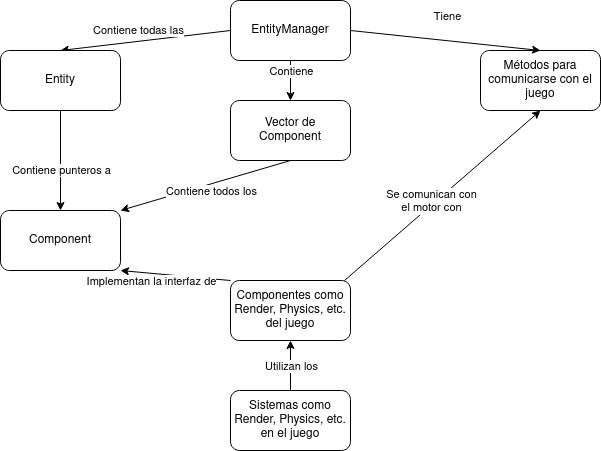
\includegraphics[width=15cm]{archivos/imagenes/Diagrama-funcionamiento-motor.png}
	\caption{Para qué se utiliza EntityManager. Diagrama de construcción propia.}
	\label{diagrama entitymanager}
\end{figure}

Como vemos en la figura \ref{diagrama entitymanager}, la clase EntityManager\_t es la clase que usará el juego para comunicarse con el motor. Tiene los métodos necesarios para almacenar, solicitar y borrar tanto entidades como un componente de una entidad. Estos componentes son almacenados en m\_components, así que EntityManager\_t tiene un fuerte acoplamiento con ComponentStorage\_t, y si quisiéramos otra implementación del motor donde los componentes no sean parte de las entidades, haría falta aplicar cambios sobre este acoplamiento.

La clase Entity\_t tiene un vector de punteros hacia sus componentes, la ventaja de esto es que no hace falta que el componente tenga un ID, y por lo tanto, la búsqueda del componente es más rápida. El inconveniente es que hay que tener mucho cuidado con dónde está almacenado el componente, ya que el encargado de darle una zona en la memoria es ComponentStorage\_t, y si este modifica la posición del componente, el puntero en Entity\_t no apuntará a la zona correcta de la memoria. 

Por último, el motor también proporciona una interfaz para la comunicación entre la entrada de teclas en el juego y el sistema operativo. Esto lo hace utilizando algunas funciones de la librería TinyPTC, que se activan cuando una tecla es pulsada.\footnote{Para un desarrollo más amplio de cómo funcionan estas funciones, ver el curso de \cite{CursoMotorC++}.}

\subsection{Dificultades a destacar}
Algunas de las dificultades de crear un motor genérico, que pueda aceptar cualquier tipo de componente es que hay que hacer las funciones template, de no ser así, cada vez que queramos añadir un nuevo componente habría que añadir una nueva función, la cual sería una copia de otra y eso podría generar errores futuros al tener que cambiar lo mismo en todas las copias. Y no solo eso, el mayor problema sería que el motor no estaría desacoplado del juego, y no sería útil para cualquier juego, sino habría que modificarlo en función del juego que queramos crear.

Un segundo problema es que la clase Entity\_t almacena punteros a Component\_t, pero como ComponentBase\_t hereda de Component\_t es posible que trabaje con los componentes del juego. ¿Por qué añadir este nivel de indirección? El problema lo hemos mencionado antes: el tipo de un componente no es un tipo básico de C++. Por lo tanto, no podremos usar una estructura de mapa para almacenar los componentes del juego según el tipo de forma lineal en memoria.
\\
Lo solucionamos de la siguiente manera: la clase Entity\_t almacena un unordered\_map de ``tipo de componente'' a ``puntero a Component\_t''. Component\_t tiene un método estático getComponentTypeID() que devuelve un entero que será el identificador único del componente durante la ejecución del programa. De esta manera, el juego podrá añadir tantos tipos de componente distintos como quiera, sin tener que preocuparse por el identificador, que es tarea del motor.
\begin{lstlisting}[style=C-color, caption={Cómo tener un número variable de componentes, sin tener que añadir un nuevo identificador con cada componente nuevo.},label=static-method]
	static ComponentTypeID_t getComponentTypeID() noexcept {
		static ComponentTypeID_t typeID { ++nextTypeID };
		return typeID;
	}
\end{lstlisting}
Pero, ¿qué significa el anterior código? Para entenderlo, hemos de saber para qué sirve la palabra reservada ``static'': cualquier variable que sea estática existirá al principio del programa, y continuará hasta el final de la ejecución del mismo. Por lo tanto, el método getComponentTypeID() devolverá siempre el mismo identificador, ya que typeID se define una sola vez en la ejecución del programa, y no cada vez que se llama al método, y nextTypeID es un miembro estático de la clase padre Component\_t que inicialmente es cero.
\\
Pero esto ocasiona el problema de que todos los componentes devolverán el mismo identificador. ¿Cómo hacemos que cada componente tenga el suyo propio? C++ tiene templates, lo que significa que, en tiempo de compilación, un código template se replicará por cada tipo diferente que haya sido instanciado la clase template. Por lo tanto, cada componente del juego, deberá heredar de ComponentBase\_t, de esta manera se crearán tantos ComponentBase\_t con su método estático getComponentTypeID() como componentes distintos tenga el juego.

Otro problema relacionado con la creación de un motor genérico es que, en algunos casos, las funciones del juego se usarán en un ámbito constante, y otras no, por lo que las funciones que queramos que sirvan para ambos casos, han de estar replicadas de forma que devuelvan un valor constante o no. El problema del código repetido que se solventa haciendo uso del las conversiones con static\_cast<>(), podemos ver un ejemplo a continuación:
\begin{lstlisting}[style=C-color, caption={Ejemplo de conversion de un método constante a no constante},label=no-constant-conversion]
	template<typename CMP_t>
	const CMP_t* getComponent() const {
		auto type = CMP_t::getComponentTypeID();
		auto it = m_components.find(type);
		if(it != m_components.end()) 
		return static_cast<CMP_t*>(it->second);
		return nullptr;
	}
	
	template<typename CMP_t>
	CMP_t* getComponent() {
		const CMP_t* cmp = const_cast<const Entity_t*>(this)->getComponent<CMP_t>();
		return const_cast<CMP_t*>(cmp);
	}
\end{lstlisting}
Hay que recordar siempre, que las conversiones han de ser de un método constante a uno no constante. De no ser así, podría suceder que el método no constante modifique algo, y devolvamos algo que ha mutado en el método constante.

\section{Segunda iteración: desarrollo del Pong}
El \textbf{29 de octubre de 2020} tuvimos la segunda iteración donde le conté a mi tutor lo que había aprendido y desarrollado, y acordamos los siguientes objetivos:
\begin{itemize}
  \item Aprender a usar \LaTeX.
  \item Comenzar la estructura de la memoria.
  \item Ver el curso de Yaser Abu-Mostafa sobre \gls{ml}.
  \item Crear un pong donde las palas se controlen aplicando aceleración y no velocidad.
  \item Almacenar los datos de la partida en \gls{csv}.
  \item Programar un perceptrón.
\end{itemize}

\subsection{Creación del juego}
Al igual que, para continuar con el desarrollo del TFG, lo primero era crear un motor funcional, antes de poder implementar los conocimientos de \gls{ia} hay que crear un juego. Como mencioné en la introducción (apartado \ref{introduccion}), esta es la parte más creativa, y puede que sea la parte que más tiempo me lleve pero no necesita prácticamente mucha formación. Por lo que, lo primero que voy a hacer es programar el clásico juego del Pong para que, posteriormente, la pala rival sea controlada por un perceptrón. 
\\
El juego tiene una estética simple, hecha sin sprites, solo coloreando en la ventana un color uniforme para cada entidad:
\begin{figure}[H]
	\centering
	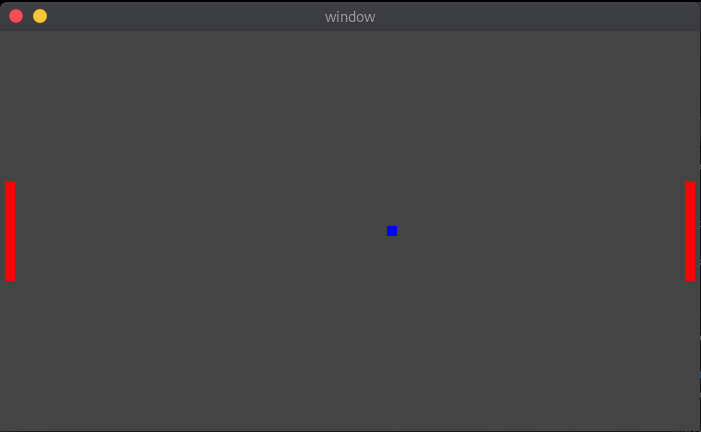
\includegraphics[width=15cm]{archivos/imagenes/pong.png}
	\caption{Imagen del primer juego, Pong.}
\end{figure}

Además, al juego le he añadido un menú, en el que eliges si quieres jugar contra un humano, para recoger los movimientos de la pala, si quieres entrenar la \gls{ia}, con algún \gls{csv} de datos de alguna partida anteriormente jugada, y una tercera opción de jugar contra una \gls{ia}. Y por supuesto la opción de salir.
\begin{figure}[H]
	\centering
	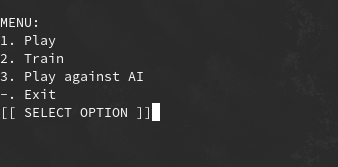
\includegraphics[width=15cm]{archivos/imagenes/menu-del-pong.png}
	\caption{Primer menú del juego.}
\end{figure}

Programar el juego no fue algo especialmente complicado, dado que durante el curso de motor de videojuegos en C++ de \citefullauthor{CursoMotorC++}, se implementan sistemas y componentes como los de colisiones, físicas, etcétera, muchos solo había que adaptarlos al Pong y ya funcionaban. Además tuve que añadir algunos extra como un sistema de puntuación, por ejemplo. Y no tuve que hacer nada de arte gráfico por el momento, ya que con unos rectángulos que se pueden generar con un for, era suficiente para entender el juego, como se puede ver en la imagen del juego.

\subsection{Resolución del resto de trabajo}
Almacenar los datos en un \gls{csv} no fue una tarea extremadamente difícil. Cada sistema tiene un método dump() y un array donde se almacenan los datos de cada frame, y cada 100 frames se guarda en un \gls{csv} los datos de ese sistema durante la partida.

La estructura de la memoria la estoy haciendo en base la plantilla que nos proporciona José Manuel Requena en GitHub \footnote{\url{https://github.com/jmrplens/TFG-TFM\_EPS}}, y fijándome en la estructura del libro de Yaser y los \gls{tfg} de mis compañeros anteriormente mencionados, de esta manera puedo tener un conocimiento de cómo escribir un documento oficial, comparando algunos anteriormente hechos.

Y por último, he comenzado a intentar implementar, sin éxito, los conocimientos sobre el perceptrón. La pala rival no responde en función de los parámetros del juego después de haber sido entrenada, por lo que estoy entendiendo mal los conceptos de \gls{ml} explicados en \citep{LearningFromData}. En la próxima cita con mi tutor le expondré este problema para ver cómo podremos darle solución.

\section{Tercera iteración: problemas con el aprendizaje}
El \textbf{26 de noviembre de 2020} volvimos a quedar para ver mi trabajo durante el último mes, y nos encontramos con varios problemas. Los problemas serían los objetivos para la próxima iteración, y fueron los siguientes.

\begin{enumerate}
	\item A pesar de tener formación en inglés y de haber cursado alguna asignatura en la carrera sobre \gls{ia}, me resultaba difícil comprender los conceptos que Yaser explicaba en el curso, así que mi tutor, me recomendó la lectura del libro en el que se basan estas charlas, en el cual se extiende más y hace más fácil la comprensión del mismo.
	\item A pesar de tener el juego del Pong ya funcionando, el día de antes estuve añadiendo código, cosa que hizo que dejara de funcionar. El código estaba bajo el control de versiones de Git, sin embargo, no sabía utilizar la herramienta por completo así que no supe volver a una versión anterior.
	\item No sabía cómo comenzar a escribir mi \gls{tfg} ni qué escribir en cada una de sus secciones.
\end{enumerate}

Después de estos problemas, ralentizamos el ritmo de desarrollo y acordamos que para la siguiente iteración: habría aprendido a usar Git por completo, habría revisado algunos de los \gls{tfg} de mis compañeros, con un posterior desarrollo del mío propio, y habría leído \textit{Learning from data: a short course} \cite{LearningFromData}

Durante esta iteración no hubo un gran avance del proyecto, debido a que todas las tareas que propusimos fue que arreglara los errores que había tenido hasta el momento, y el tiempo entre esta y la siguiente era más reducido de lo normal.

\section{Cuarta iteración: juego con el perceptrón}
El \textbf{17 de diciembre de 2020} tuvimos la última cita del año, revisamos los objetivos marcados en la anterior iteración y ya había desarrollado brevemente cada campo de la memoria del \gls{tfg}, implementado el perceptrón y aprendido a usar Git. Sin embargo, no habiendo terminado de leer \textit{Learning from data: a short course}, y con las ideas un poco confusas, el perceptrón no respondía correctamente, por lo que los objetivos para la siguiente iteración serían:
\begin{itemize}
  \item Completar toda la memoria con las cosas hechas hasta el momento.
  \item Ver las clases de Razonamiento Automático de mi tutor.
  \item Arreglar la implementación del perceptrón.
  \item Hacer funcionar el perceptrón dentro del juego.
  \item Rehacer el sistema de recogida de datos en \gls{csv}.
\end{itemize}

\subsection{Desarrollo total del perceptrón}
El problema principal con el perceptrón fue que, debido a algunas similitudes entre entrenar y jugar, implementé el código de tal forma que todo estaba en la misma clase. Mi tutor me explicó que la parte del entrenamiento está separada del juego y me dijo que viese las clases de Razonamiento Automático, de esta manera conseguiría aclarar las ideas tan dispersas que tenía.

Lo que hace el perceptrón es recibir los datos relevantes de la partida, como son las físicas de la pelota y del jugador controlado por la \gls{ia}. Entonces, los datos son una X de la fórmula \ref{suma ponderada}, los pesos del perceptrón ya entrenado son representados con una W, y el número total de datos es N.
\begin{equation}
	\sum_{i=0}^NX_{i}*W_{i}
	\label{suma ponderada}
\end{equation}
El resultado de ese sumatorio será positivo o negativo, y no es necesario añadir en la fórmula el límite, sino que el límite es 0 ya que entre los datos se ha añadido el threshold como una entrada con valor 1, y entre los pesos se ha añadido uno extra al principio para que se ajuste al igual que el resto de pesos. En el caso de dar positivo, significará que la suma ha superado el threshold (representado como $w_o(t)$ en la figura \ref{perceptron}), lo que significa que la \gls{ia} manda al juego pulsar esa tecla de la pala, y en caso de ser negativo no. A cada tecla (arriba y abajo) le corresponde un perceptrón, que es el que decide si esta es pulsada o no.

Para entrenar al perceptrón, paso previo para jugar contra él porque sino, no existirá un fichero con la configuración del mismo, lo que hago es:
\begin{enumerate}
	\item Generar un array de pesos aleatorios y calcular el error que generan estos pesos.
	\item Se repite N veces el siguiente proceso:
	\begin{enumerate}
		\item Se calcula el error de los pesos que se quiere ajustar.
		\item Si este perceptrón con estos pesos es mejor que el mejor hasta el momento (tiene un error menor), se guarda.
		\item Del perceptrón ajustado, se elige uno al azar entre todos los puntos que no ha acertado si pulsar o no pulsar. 
		\item Si la tecla no fue pulsada, y debía serlo, se suma al peso el valor del input del perceptrón. Si la tecla fue pulsada, y no debía serlo, se resta. (Es decir, teniendo M entradas, la operación de suma o resta se hace desde 0 hasta M, al peso i se le suma/resta el input i).
	\end{enumerate}
	\item El perceptrón que haya dado menor error se guarda en un fichero para poder ser usado en el juego.
\end{enumerate}

El perceptrón ya funcionaba correctamente después de ver las primeras clases de Razonamiento Automático, ya que conseguí entender las dudas que me quedaban sobre el tema. Dando un resultado totalmente jugable, ya que no era invencible, ni tampoco tan malo como para no convertirse en un reto. El error que no permitía funcionar de forma correcta era una mala proporción de los datos entregados al agente durante el entrenamiento. El \gls{csv} de datos tenía una cantidad mucho mayor de ejemplos de ``no pulsar'', y muy pocos de ``sí pulsar'', por lo que en la mayoría de casos, el perceptrón entrenado se quedaba parado. Esto tenía varias posibles soluciones, entre ellas ajustar el cálculo del error (es decir, que un fallo de no pulsar cuando sí hay que hacerlo subiese más el valor error), y por la que opté yo, que era ajustar los datos de tal manera que quedasen distribuidos la mitad del ejemplo de frames pulsando y la otra mitad no pulsando. Esto trajo otro pequeño inconveniente, y era que los datos extraídos de ``no pulsar'' eran del principio de la partida, y esos frames de ejemplo no eran lo suficientemente representativos, por lo que opté por coger los frames aleatorios.

\subsection{Desarrollo de una red neuronal}
Además, en las clases de Razonamiento Automático, Francisco J. Gallego-Durán explica cómo funciona una red neuronal y cómo programarla, incluso, invita a los alumnos a crearla de tal forma que sea diferente a la ya creada por él, sin el uso de la librería vector de C++ para conseguir una mayor eficiencia en lo que se refiere a los tiempos de ejecución. Por lo que después de aprender los conceptos con sus clases, me dispuse a programar mi propia red neuronal para después introducirla en el juego cuando este se convirtiera en algo más complejo que una pala rebotando una bola, sin embargo, no era consciente de las facilidades que aporta la clase vector, y me topé con varios problemas durante el desarrollo.
\\
Algunos de estos problemas fueron, tener que sobrescribir el constructor de copia por no comportarse cómo deseaba, tener que manejar el puntero de los datos según si se quería contar el threshold o no (recordemos que uno de los motivos por los que haría una implementación propia de la clase vector sería para obtener más eficiencia a la hora de leer los datos), etc.
\\
El hecho de tener que detenerme a estudiar cómo funcionan algunas de las facilidades que aporta vector, y escribir las partes de la memoria que faltaban me llevó todo el tiempo que quedaba hasta esta quinta iteración. Ya había solventado los problemas de la anterior y había alcanzado los objetivos propuestos, por lo que llegué con todo el trabajo hecho a esta.

\subsection{Recogida de datos de la partida}
Además, un segundo problema de concepto fue el cómo recoger los datos. En primera instancia cada sistema se encargaba de recoger sus datos en el \gls{csv}, de tal manera que como los sistemas necesarios para que la \gls{ia} aprenda son las físicas y el sistema de input, había dos archivos que correspondían a la misma partida, con distinto nombre y distintos datos, pero tremendamente acoplados, por lo que mi tutor sugirió que los recoja de manera externa a sus sistemas, todos los datos necesarios en un mismo \gls{csv}, así que ese era otro objetivo para la siguiente iteración. 

Y por último, me dijo que no era necesario almacenar datos en array e intentar optimizar la escritura de estos datos en un fichero, ya que el juego no es tan complejo como para que se ralentice por abrir y escribir un archivo en cada frame. Conseguí solucionarlo rápidamente. Al principio de la partida creo unas referencias a los objetos que necesito guardar, y en cada frame abro el archivo y lo escribo con los datos actuales. No es la forma más eficiente de hacerlo, pero para un juego tan sencillo funciona perfectamente.

\section{Quinta iteración: mejorando el juego}
El \textbf{14 de enero de 2020} tuvimos la siguiente iteración, los objetivos marcados para la siguiente iteración han sido más ambiciosos de lo normal, así que no es necesario que estén completos, pero mi tutor comentó que sería bueno al menos intentarlo, de tal manera que fueron:
\begin{enumerate}
	\item Arreglar algunos defectos de la memoria debidos a mi falta de experiencia escribiendo documentos oficiales.
	\item Desarrollar el Pong Plus, un juego inspirado en el Pong, pero con ciertos añadidos que lo hacen más complejo
	\begin{itemize}
		\item Minions en el centro del campo (pequeñas palas que ayudan a su compañero a ganar).
		\item Los minions son capaces de rebotar la pelota, y su movimiento es solo en el eje y.
		\item Los minion pueden morir a causa de un disparo, de ser así reaparecerán tras unos segundos.
	\end{itemize}
	\item Añadir un sistema de recogida de datos que tenga en cuenta los nuevos datos de la partida, y que también funcione para los minions.
	\item El jugador debe poder elegir si jugar con la pala o con el minion, para así obtener el correspondiente \gls{csv} que servirá de entrenamiento.
	\item Añadir una opción para poder configurar el entrenamiento recibido desde el juego.
	\item Portar el juego para Windows, dado que actualmente solo está compilado para Linux.
\end{enumerate}

\subsection{Pong Plus}
Lo primero que hice esta vez fue: cambiar los colores del juego, añadir un marcador dentro de la pantalla y una linea en medio, para intentar mejorar la estética del juego. El resultado está en la figura \ref{primera vista del pong plus}.

\begin{figure}[H]
	\centering
	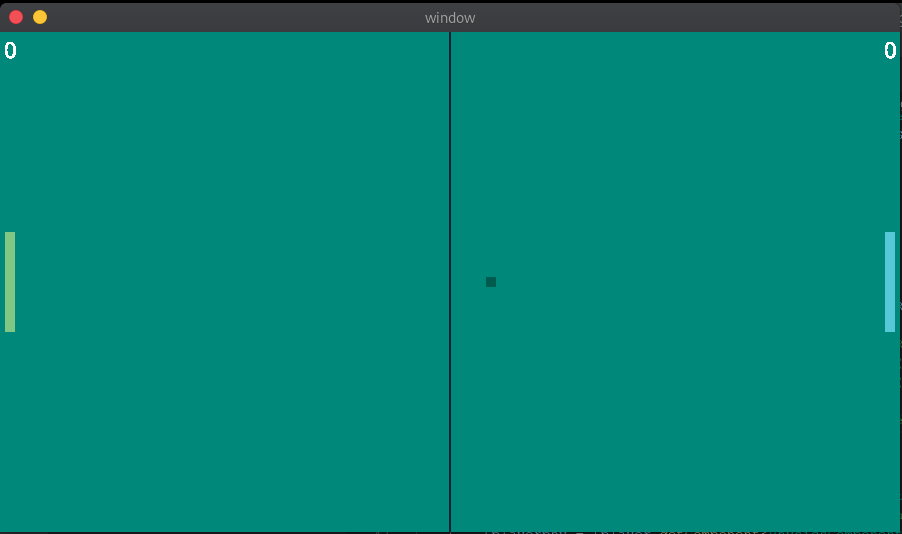
\includegraphics[width=12cm]{archivos/imagenes/pong-nuevos-colores.png}
	\caption{Imagen del Pong con nuevos colores y marcador.}
	\label{primera vista del pong plus}
\end{figure}

Lo que hice en segunda instancia, no estaba dentro de los objetivos que nos habíamos marcado pero decidí hacer un menú, pensando que sería algo sencillo, pero me llevó más tiempo del que imaginaba. Para hacer el menú necesitaba renderizar texto, y para no alargar más el desarrollo, decidí añadir una librería que se usa para renderizar texto en formato true type llamada stb\_truetype\footnote{La librería es del tipo conocido como only-header, se encuentra en github junto con otras utilidades \url{https://github.com/nothings/stb}}. De esta manera, también podría usar los números del marcador como texto. Para moverte por el menú se usarán las flechas del teclado de arriba y abajo. El resultado lo puedes ver en la figura \ref{primer menu del juego}.

\begin{figure}[H]
	\centering
	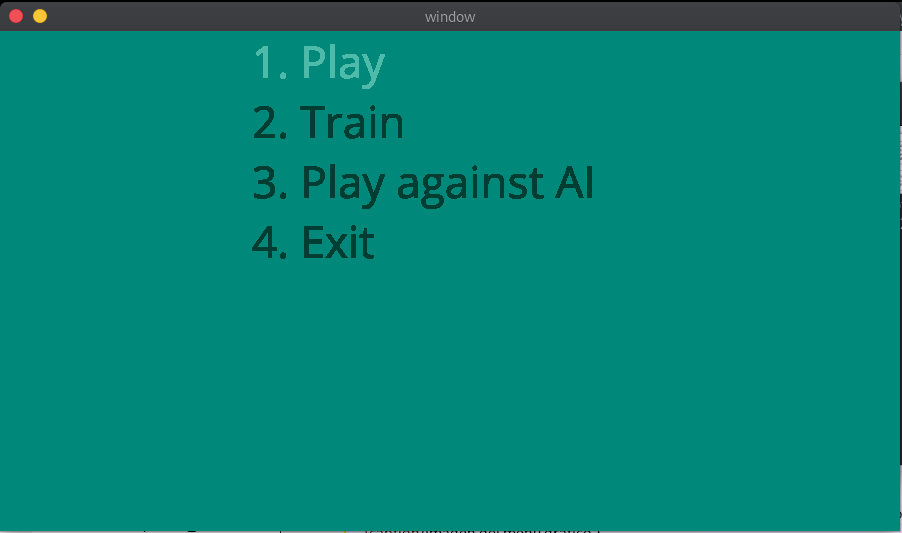
\includegraphics[width=12cm]{archivos/imagenes/menu-grafico-integrado-en-el-juego.png}
	\caption{Imagen del menú gráfico.}
	\label{primer menu del juego}
\end{figure}

Una vez acabado el menú, que además te permite seleccionar qué \gls{csv} quieres usar entre todos los que has generado jugando, añadí los minions y unas paredes, las cuales habría que romper para poder pasar tu bola al campo enemigo. Esto es posible porque las bolas traspasan las paredes que son de su mismo color.

\begin{figure}[H]
	\centering
	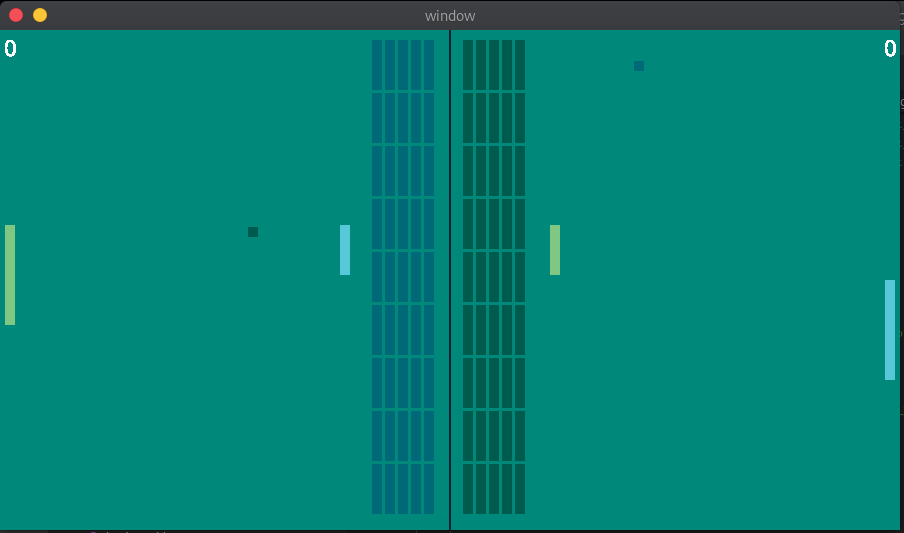
\includegraphics[width=12cm]{archivos/imagenes/pong-plus-con-minions-y-paredes.png}
	\caption{Imagen de la primera versión del Pong Plus.}
\end{figure}

\subsection{Compilación para Windows}
Lo último que hice en este periodo fue compilar el juego para Windows. Mi tutor explica en el curso de videojuegos \cite{CursoMotorC++} cómo modificar el fichero de construcción (Makefile) para compilar para Windows desde una máquina con Linux (comúnmente conocido como cross-compiling), y en la librería de TinyPTC descargable, también hay unos ficheros de código específicos para Windows, por lo que la única tarea que me quedaba por hacer era modificar las partes del código donde se incluye la versión de TinyPTC de Linux e incluir la versión de Windows, y recompilar el proyecto. 
\\
Pero cuando probé el juego en Windows, se ejecutaba correctamente, pero no respondía ante la entrada por teclado. Y es que la codificación del teclado en Windows no es la misma que la de X11, por lo que creé un fichero en el que definí los valores de la variable dependiendo de si la compilación está activada para Windows o para Linux. Posteriormente usé ``\#ifdef''\todo{Aquí tampoco sé si usar cursiva, comillas... o qué usar} que hace que el compilador use esa parte del código sólo se compile si la macro está presente en la linea de compilación, o si está definida previamente en otro fichero incluido por este, de esta manera lo podía combinar con ``\#else'' para definir las teclas del juego para Windows cuando construya el juego para Windows, y las teclas de Linux cuando compile para este sistema operativo.

\section{Sexta iteración: aprendizaje mediante backpropagation}
\label{sexta iteracion}
El \textbf{11 de febrero de 2021} tuvimos una nueva reunión, en la cual los objetivos marcados fueron:
\begin{enumerate}
	\item Continuar mejorando defectos de la memoria y desarrollando los nuevos hitos de las nuevas iteraciones.
	\item Implementar Dear ImGui en el proyecto
	\begin{itemize}
		\item Estudiar cómo se usa.
		\item Sustituir TinyPTC por OpenGL3 para poder renderizar tanto el juego como las ventanas.
		\item Diseñar menús para manejar el juego.
	\end{itemize}
	\item Programar el algoritmo de backpropagation.
	\item Poder elegir tanto los ficheros de datos de entrenamientos como los ficheros de pesos para el juego.
	\item Añadir un campo de entrenamiento para que no sea necesario que haya dos jugadores para recoger datos de entrenamiento.
	\item Añadir un algoritmo básico para cuando no exista un fichero de pesos pero que se pueda jugar contra una \gls{ia}.
\end{enumerate}

Comencé la iteración con ilusión, viendo documentación de Dear ImGui y estudiando cómo implementar la librería en mi proyecto. Pero antes de empezar a implementarlo debía acabar lo que empecé en la anterior iteración, la red neuronal. Es cierto que en la anterior iteración la red neuronal ya era capaz de resolver el problema de la XOR con un entrenamiento aleatorio, es decir, probar una asignación de pesos aleatoria para la red, y si obtenía mejores resultados que la mejor red hasta el momento, se sustituían los pesos de la red neuronal por estos nuevos.
\begin{figure}[H]
	\centering
	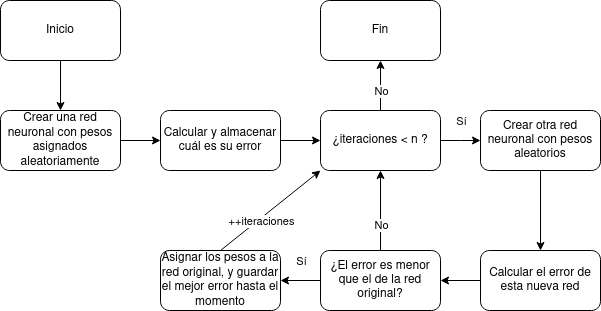
\includegraphics[width=15cm]{archivos/imagenes/Algoritmo-red-neuronal-aleatorio.png}
	\caption{Algoritmo de aprendizaje aleatorio. Esquema de construcción propia.}
	\label{Algoritmo aleatorio}
\end{figure}
Es un algoritmo que podría funcionar en algunos casos, pero requiere de un número mucho más alto de iteraciones de media, así que no es lo suficientemente eficiente. Por lo que me dispuse a desarrollar el algoritmo de backpropagation.

\subsection{Desarrollo de Backpropagation}
Durante esta iteración apliqué Backpropagation a la red neuronal ya creada antes, como puedes ver en el apartado \ref{marco teorico backpropagation}, y me di cuenta de un grave error que cometí desarrollando la red neuronal, como se puede apreciar en el apartado \ref{aleatorio vs backpropagation resultados}, comparo la velocidad a la que aprende la red neuronal usando los dos diferentes tipos de entrenamiento, y originalmente las conclusiones que saqué fueron las siguientes:
\\
El algoritmo aleatorio consigue aprender más rápido que el de backpropagation porque el problema de la puerta XOR es demasiado sencillo, y por lo tanto la estructura de la red es demasiado simple. Llegando a concluir que el algoritmo aleatorio encuentra la solución el 80\% de las veces después de iterar 1000 veces, mientras que el algoritmo de backpropagation encuentra la solución sólo el 1.4\% de las veces, y para llegar al 80\% habría que iterar 100000 veces. Cuando le comenté estas conclusiones a mi tutor me dijo que era muy extraño que una red neuronal tardara tanto en aprender el problema de la XOR, siendo tan simple la estructura de la red (dos neuronas de entrada, una capa oculta con cuatro neuronas, y una de salida). Para hallar estos datos ejecuté cada uno de los anteriores experimentos 10000 veces y así conseguir que la media fuese algo significativo, y que la varianza afectase lo mínimo posible.

¿Dónde se encontraba el problema? No parece una conclusión lógica. El problema, como recuerdo en la cita del principio de esta memoria, estaba entre la silla y el teclado. Y es que había programado mal el constructor de la clase de la red neuronal, este asignaba mal los punteros de una capa de la red a su siguiente capa. De tal forma que para calcular el delta de backpropagation sólo se calculaba bien en la última capa, que no depende de ninguna capa posterior, por lo tanto sólo variaban los pesos de las neuronas de la última capa, y por eso era tan costoso que la red aprendiese, porque el resto de capas se quedaban con el valor inicial aleatorio y no variaban en todo el entrenamiento. En la figura \ref{problema aprendizaje red neuronal} puedes ver un ejemplo ilustrativo del problema.
\begin{figure}[H]
	\centering
	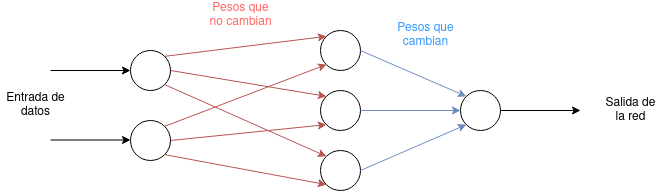
\includegraphics[width=15cm]{archivos/imagenes/problema-de-aprendizaje-red.png}
	\caption{Problema de aprendizaje de la red neuronal.}
	 \label{problema aprendizaje red neuronal}
\end{figure}

\section{Séptima iteración: creación de menús}
El día \textbf{11 de marzo de 2021} volvimos a tener una llamada de revisión de trabajo y nuevas propuestas, pero según se desarrolló la anterior iteración, mi tutor y yo acordamos que para esta acabaría lo ya acordado, prestando especial atención en el desarrollo de la memoria, ya que era lo que más trabajo requería en la situación en la que estaba, y conociendo que ya quedaba poco tiempo para la entrega del \gls{tfg}.

\subsection{Dear ImGui}
Por lo tanto, comencé a implementar Dear ImGui en el proyecto. El primer paso era sustituir TinyPTC por OpenGL3, así que eso hice: fui al sistema de Render, que se encarga de abrir la ventana y dibujar sobre ella, y cambié todo el código necesario en este punto. Ahora la ventana la abriría con OpenGL3 y cada frame dibujado por software mediante el sistema de render se pasaría a OpenGL3 también, de esta manera Dear ImGui solo tendrá que dibujar las ventanas encima de mi interfaz.
\\
El siguiente paso fue aprender a dibujar una ventana dentro del juego, y así fue, algo bastante sencillo porque aparece en el código de ejemplo que ellos tienen en el proyecto.

\begin{figure}[H]
	\centering
	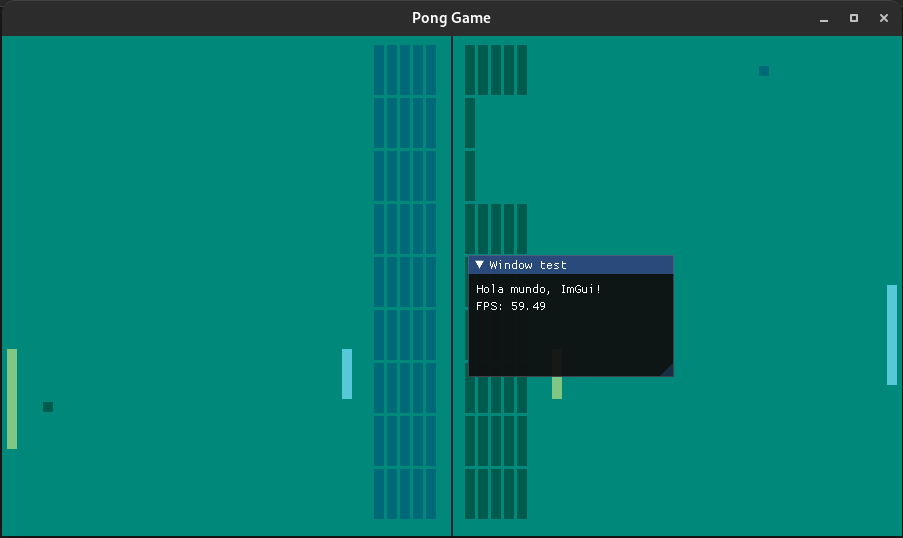
\includegraphics[width=15cm]{archivos/imagenes/ventana-dentro-del-juego.png}
	\caption{Ventana dentro del juego.}
\end{figure}
Pero como los menús de los juego no suelen ser en una ventana, decidí hacerlo en pantalla completa. No es el mejor diseño, pero ya servía para poder manejarse  dentro del juego.
\begin{figure}[H]
	\centering
	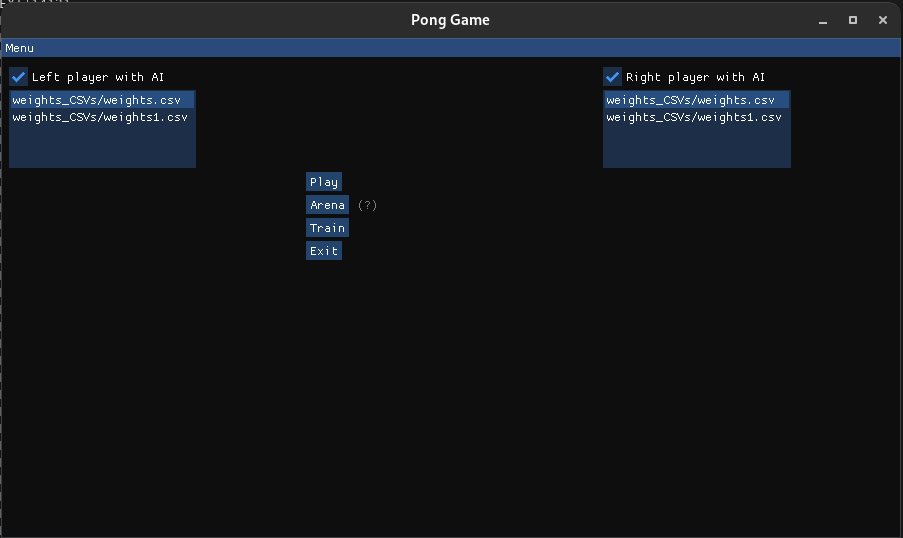
\includegraphics[width=15cm]{archivos/imagenes/menu-del-juego.png}
	\caption{Menú del juego.}
	\label{Menu del juego}
\end{figure}
Ahora ya, teniendo las herramientas que nos da Dear ImGui, me dispuse a desarrollar un menú en el cuál el jugador, pueda decidir cómo entrenar a su \gls{ia}, y además que pueda ver de manera gráfica cómo va aprendiendo y cuáles son las consecuencias de cambiar los parámetros de entrenamiento de la \gls{ia}. Puedes ver el menú de entrenamiento en la figura \ref{Menu de entrenamiento}.

\subsection{Campo de entrenamiento}
El campo de entrenamiento es el apartado de arena que puedes ver en la figura \ref{Menu del juego}, que te pondrá a jugar en el mismo campo de siempre, pero sin rival, cuando la pelota llega a la pared del rival rebotará, de esta manera el jugador podrá reaccionar a diferentes situaciones de partida (con el minion rival en una posición, las bolas en otras posiciones, con velocidades distintas, etc.) que servirán como dataset para un posterior entrenamiento en el menú de entrenamiento.
\begin{figure}[H]
	\centering
	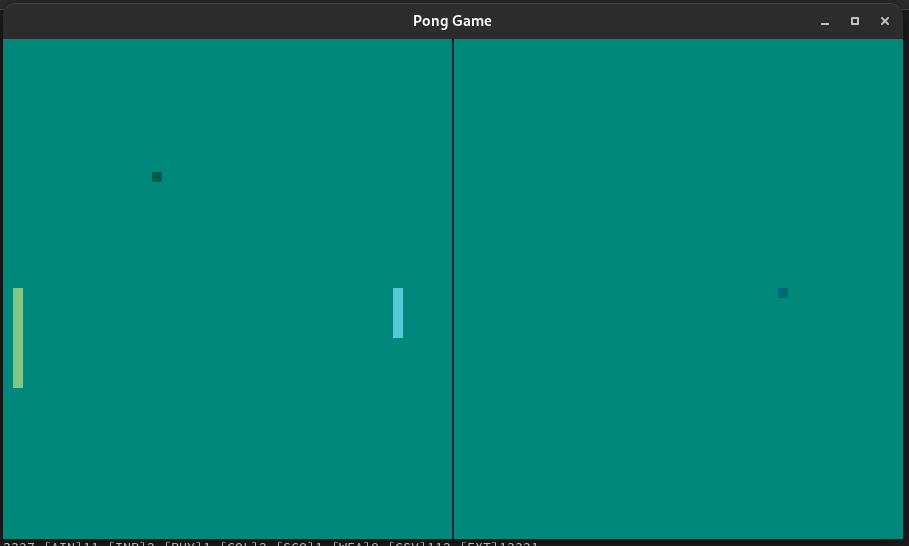
\includegraphics[width=15cm]{archivos/imagenes/arena-de-entrenamiento.png}
	\caption{Arena de entrenamiento.}
\end{figure}

Después de obtener todos los datos podremos ir al siguiente menú de la figura \ref{Menu de entrenamiento}, donde el jugador elegirá los parámetros que considere oportunos para entrenar la \gls{ia}. Entre ellos podrá cambiar, la cantidad de muestras que usa de cada tipo (de esta manera soluciono el problema ya conocido desde la neurona, y es que hay una gran cantidad de ejemplos de no tocar en la muestra), el ratio de aprendizaje que aplicará, la estructura de la red neuronal, y por supuesto, el número de iteraciones que hará Backpopagation. Por último, abajo del todo se puede apreciar una gráfica en la cuál pone a su derecha "\% of error". En esta gráfica el usuario verá el progreso de cómo va disminuyendo el error a lo largo del tiempo.
\begin{figure}[H]
	\centering
	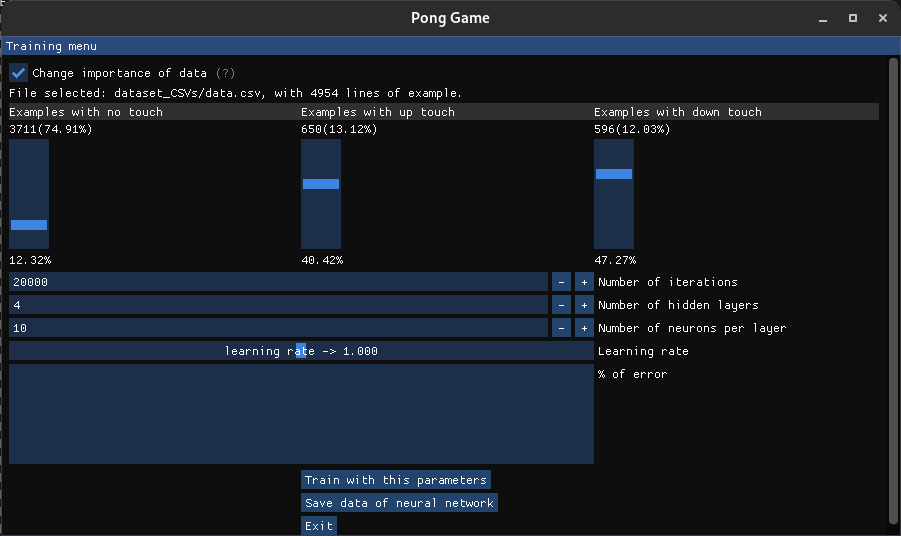
\includegraphics[width=15cm]{archivos/imagenes/menu-de-entrenamiento.png}
	\caption{Menú de entrenamiento del juego.}
	\label{Menu de entrenamiento}
\end{figure}

\section{Octava iteración: perfilando el proyecto}
\label{octava iteracion}
El \textbf{13 de abril de 2021} ya solo quedaba un mes para la confirmación de la entrega del proyecto en el C3, por lo que ya tendríamos que tener todo acabado para la siguiente fecha, o a punto de acabar para confirmar la entrega. Los objetivos para esta iteración, por lo tanto, fueron los siguientes:
\begin{enumerate}
	\item Añadir capturas a la memoria, puesto que eran escasas y eran necesarias para entenderla.
	\item Añadir apartado de resultados a la memoria, con tablas, imágenes, y demás representaciones.
	\item Arreglar el método de entrenamiento de la \gls{ia}.
	\item Añadir un algoritmo básico para cuando no exista un fichero de pesos pero que se pueda jugar contra una \gls{ia}.
\end{enumerate}

\subsection{Arreglo del entrenamiento}
Cuando desarrollé el algoritmo de aprendizaje de la red neuronal inicialmente, decidí añadir un factor de importancia a cada acción (pulsar arriba, abajo, o no pulsar). Esto fue porque ya tuve problemas inicialmente con el perceptrón y sé que la cantidad de ejemplos de cada tipo está desproporcionada, ya que existe mayor cantidad de ejemplos de no pulsar, respecto a los que sí hay una pulsación de tecla.
\\
Como el algoritmo de Backpropagation ya estaba programado, decidí que en la última capa el delta se multiplicase por el porcentaje de importancia que le diera el usuario, pero aparentemente no funcionaba. En la reunión con mi tutor me explicó que multiplicar el delta destrozaba el aprendizaje, que lo que tendría que hacer realmente era escoger de forma aleatoria, con una probabilidad (la que el usuario ha asignado en el menú de entrenamiento), los elementos de la muestra. Posteriormente, desordenar el vector de frames obtenido para que la red neuronal no aprenda los últimos movimientos de la partida, por culpa de la corrección de Backpropagation, ya que es un problema conocido que tras un número alto de iteraciones la red puede aprender el ruido de la muestra y generalizar mal fuera de ella.

\begin{figure}[h]
	\centering
	\begin{subfigure}[h]{\textwidth}
		\centering
		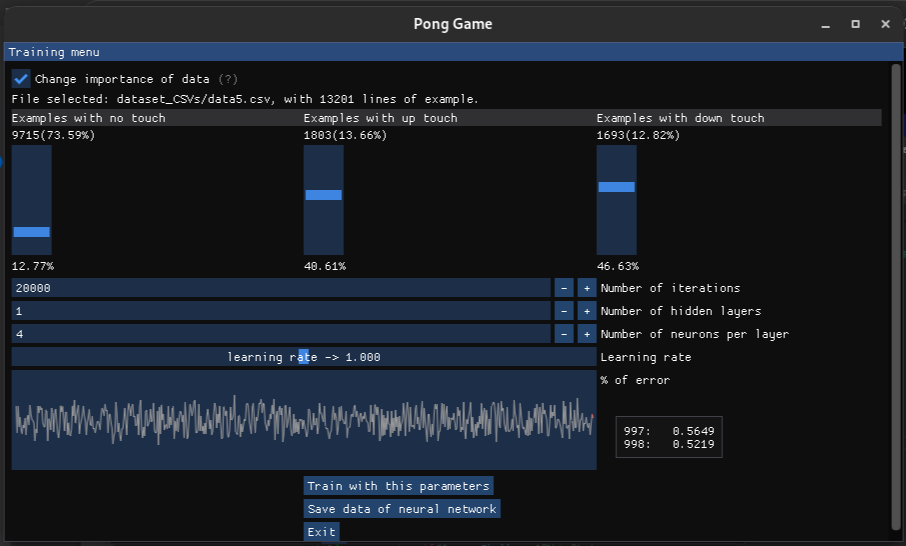
\includegraphics[width=15cm]{archivos/imagenes/menu-de-entrenamiento-alto-error.png}
		\caption{Alta importancia a pulsar.}
	\end{subfigure}

	\begin{subfigure}[h]{\textwidth}
		\centering
		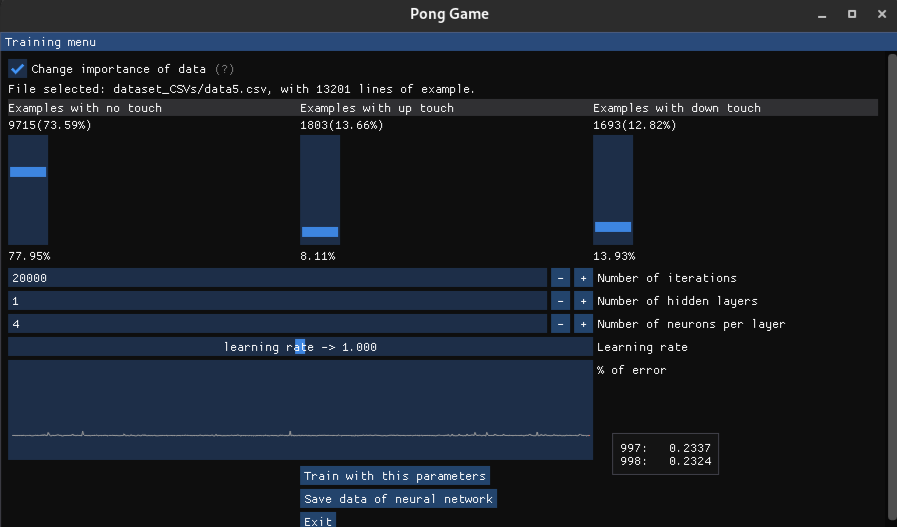
\includegraphics[width=15cm]{archivos/imagenes/menu-de-entrenamiento-bajo-error.png}
		\caption{Baja importancia a pulsar.}
	\end{subfigure}
	\caption{Comparación entre las importancias de pulsar o no pulsar.}
	\label{Comparacion alto vs bajo error}
\end{figure}

Además, la gráfica que representaba el porcentaje de error de la red neuronal de forma genérica era poco representativa, porque como vemos en la figura \ref{Comparacion alto vs bajo error}, cuando intentas que la red neuronal se comporte mejor en partida aumentando la importancia de pulsar, el error aumenta desde el 50\% hasta el 70\%. Mientras que, si lo que aumento es la importancia de no tocar (teniendo en cuenta que representa el 75\% del dataset), el error de la red permanece entre el 20\% y el 23\%. Esto puede dar una falsa imagen al usuario de que la red no está aprendiendo, por eso he separado en dos gráficas, el error que comete respecto a los ejemplos de no tocar, y el error que comete respecto a los ejemplos de sí hacerlo (figura \ref{menu dos graficas}).

\begin{figure}[H]
	\centering
	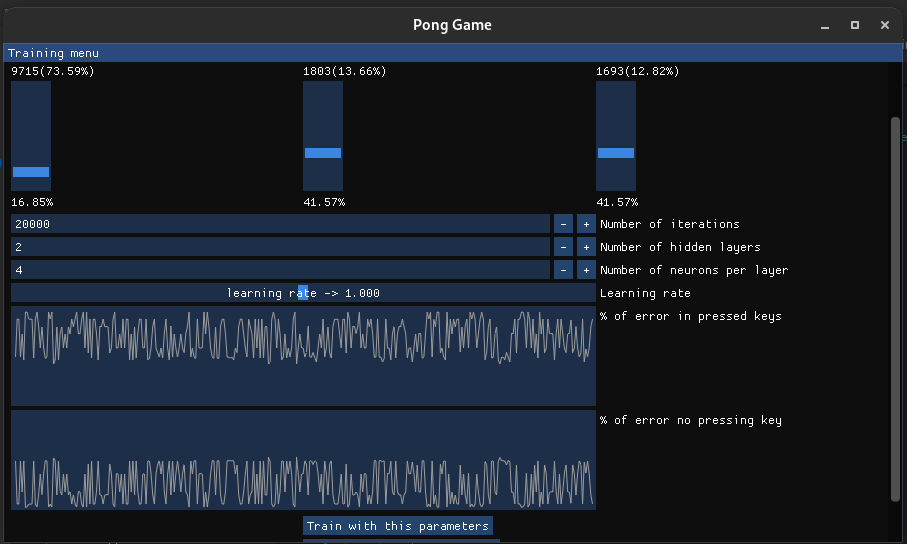
\includegraphics[width=15cm]{archivos/imagenes/menu-de-entrenamiento-dos-graficas.png}
	\caption{Menú con dos gráficas para comparar error de pulsar y no pulsar.}
	\label{menu dos graficas}
\end{figure}

\subsection{Algoritmo básico de seguimiento}
Como el usuario no tendrá ningún fichero de pesos, este necesitará un algoritmo para poder jugar contra la máquina, para poder entrenar a su bot. Por lo tanto, mi tutor y yo tuvimos la idea de darle un algoritmo por defecto a los caracteres controlados por la máquina. Escribiré un pseudocódigo para una mayor facilidad de comprensión del mismo:
\begin{lstlisting}[style=C-color, caption={Pseudocódigo de algoritmo de IA diseñada},label=pseudo-code-ia-designed]
	Entity myself     = getMyself();
	Entity leftBall    = getLeftBall();
	Entity rightBall = getRightBall();
	
	if( (myself.x - leftBall.x)*(myself.x - leftBall.x) < 
		(myself.x - rightBall.x)*(myself.x - rightBall.x)) { //leftBall is closer
		if((myself.y - leftBall.y) > 0)
			pressDown();
		else
			pressUp();
	} else {
		if((myself.y - rightBall.y) > 0)
			pressDown();
		else
			pressUp();
	}
\end{lstlisting}
Aunque el código consta de varias lineas, es extremadamente sencillo de explicar: busca la pelota más cercana, y si está por encima en el eje y, pulsa hacia arriba. En caso contrario, hacia abajo. Desde luego no es el algoritmo más eficaz, entre otros problemas porque cuando pulsas no te mueves, sino que aceleras, pero es un sencillo algoritmo que servirá para responder algunas de las bolas antes de que el usuario haya entrenado su primera red neuronal.
 
\section{Novena iteración: los retoques finales al proyecto}
\label{novena iteracion}
El día \textbf{6 de mayo de 2021} fue la última iteración antes de decidir si entregaríamos el \gls{tfg}. Efectivamente, decidimos que sí lo haríamos, sin embargo, quedaba un duro trabajo en el mes de mayo, para acabar todas las cosas que quedaban por terminar y tener una memoria y un proyecto finalmente dignos de ser presentados ante el tribunal. Los objetivos, por lo tanto, fueron:
\begin{enumerate}
	\item Detectar y corregir el error de aprendizaje en el juego.
	\begin{itemize}
		\item Comprobar que los datos de entrada y salida se están dando bien a la red.
		\item Revisar manualmente los cálculos para algunos ejemplos.
	\end{itemize}
	\item Diferenciar entre ``gradient decent'' común y ``stochastic gradient decent''.
	\item Explicar el error en la memoria.
	\item Escribir las conclusiones en la memoria.
\end{enumerate}

El problema del aprendizaje en el juego ya había sido solventado en la octava iteración en el apartado \ref{octava iteracion}, mientras que el problema de errores en la programación ya había sido resuelto en la sexta iteración, en el apartado \ref{sexta iteracion}. Entonces, ¿qué es lo que había que corregir? ¿Por qué la red no es capaz de aprender con los datos que le aporta? Por esto es que marcamos el objetivo de ``Detectar y corregir el error de aprendizaje en el juego''.

Para mayor claridad, añadí una tercera gráfica, para ver si lo que aprendía era pulsar hacia arriba o hacia abajo. Además de un cálculo de cuántos pesos tiene en total la red, para poder determinar la dimension Vapnik-Chervonenkis, y cuántos ejemplos de cada tipo se están cogiendo en lugar de su porcentaje para mayor claridad (anteriormente era el porcentaje, pero esto aparece ahora cuando la barra es pulsada, y lo que aparece abajo es el número de muestras que tendrá de cada tipo). Figura \ref{ultimo menu de entrenamiento}.
\begin{figure}[H]
	\centering
	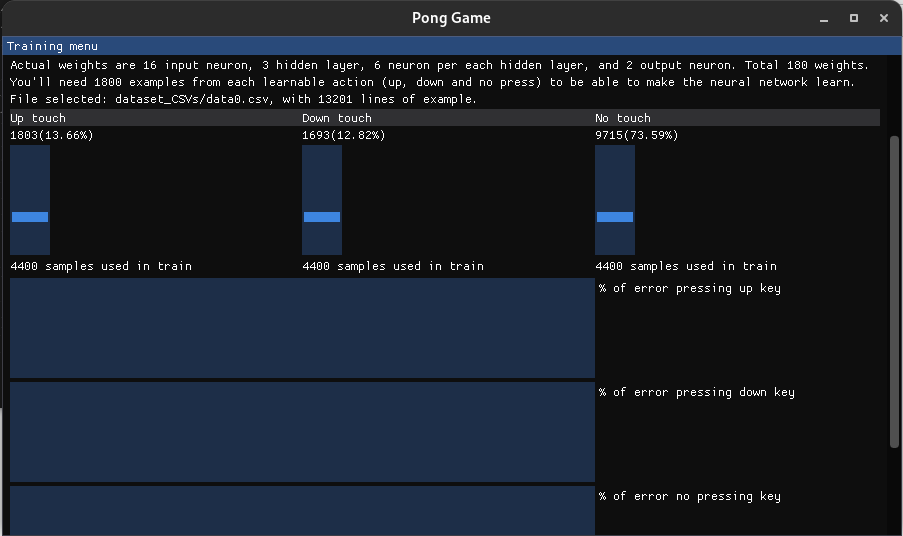
\includegraphics[width=15cm]{archivos/imagenes/menu-de-entrenamiento-definitivo.png}
	\caption{Menú de entrenamiento definitivo.}
	\label{ultimo menu de entrenamiento}
\end{figure}

Con todas las herramientas diseñadas me puse a investigar sobre los posibles errores tanto en el código (revisar las lecciones para ver si había tenido algún error de concepto), como en las muestras que se le entregan (que estuviese bien distribuido), y no encontraba ningún error. Lo más llamativo era el comportamiento de las gráficas, pues por lo general, el error de cada uno de los tipos pasaba de 100\% a 0\% de golpe entre el error denominado como "pulsar", ya sea en la tecla hacia arriba y en la tecla hacia abajo, mientras que cuando uno de estos dos pasaba a 0\% de error, el denominado como "no pulsar" pasaba a ser del 50\%. Puedes ver un ejemplo de esto en la figura \ref{error erratico}.
\begin{figure}[H]
	\centering
	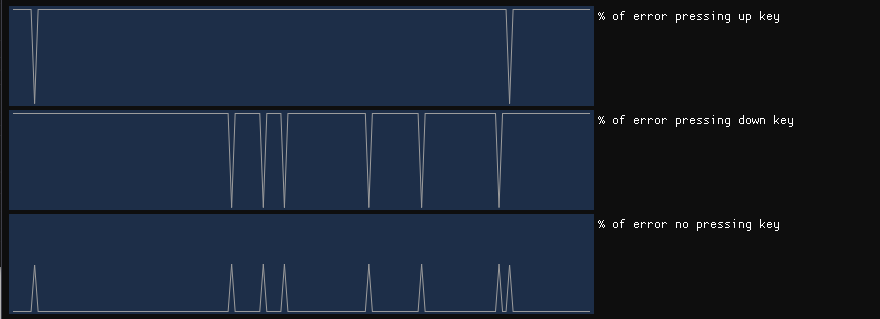
\includegraphics[width=15cm]{archivos/imagenes/error-erratico.png}
	\caption{Variación del error confusa.}
	\label{error erratico}
\end{figure}

Era, cuanto menos, curioso. Después de un tiempo probando y cambiando los distintos parámetros, conseguí que esto ya no fuera así. Usé una red más compleja que la que estaba usando comúnmente, un 20\% de ejemplos de no tocar frente al 80\% de sí hacerlo, una cantidad de iteraciones más alta, y un ratio de aprendizaje ridículamente bajo comparado con lo que estaba usando hasta ahora (acostumbrado a variar entre cero y dos, pero lo más normal era uno), 0.00185. La red comenzó a bajar el error en los tres tipos poco a poco, y no a saltos agigantados, como se aprecia en la figura \ref{error concordante}. Por lo tanto, llegué a la conclusión de que estaba aprendiendo, cosa que confirmé luego poniéndolo a prueba en el juego.
\\
Por supuesto, después de conocer el por qué del error, el rango de ratio de aprendizaje pasó de entre cero y dos, a entre cero y uno. Haciendo especial énfasis en los valores más cercanos a cero, por lo tanto ahora la barra para elegir el ratio de aprendizaje avanza de forma logaritmica (para tener más precisión con los números pequeños), en lugar de la anterior forma uniforme.
\begin{figure}[H]
	\centering
	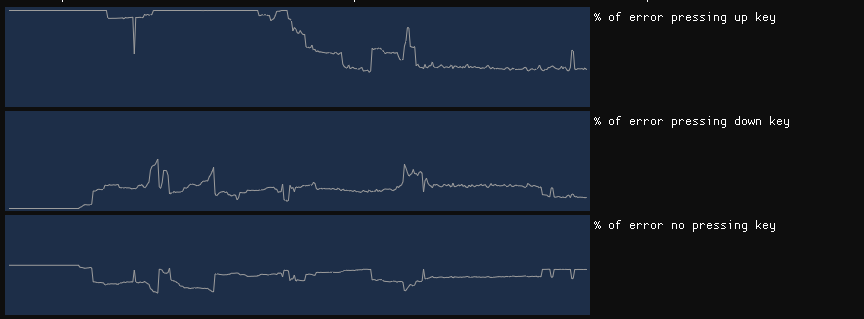
\includegraphics[width=15cm]{archivos/imagenes/error-concordante.png}
	\caption{Variación del error concordante.}
	\label{error concordante}
\end{figure}

Sin embargo, aunque ahora la red neuronal es capaz de jugar, noto que la forma en la que juega es más errática que cuando era controlada por un perceptrón, incluso más errática que el algoritmo de \gls{ia} diseñada simple que hice. Hablaré más sobre ello en el apartado de conclusiones (apartado \ref{conclusiones}).

Respecto al descenso del gradiente, estuve revisando las diferentes fuentes de información que he utilizado durante el proyecto, y he comprendido la diferencia con el modelo estocástico. Es posible que ese sea el motivo por el que la red neuronal es más errática de lo que debería. La diferencia entre el modelo común y el estocástico es que en el descenso del gradiente común, se hace la media de todos los errores de la muestra, y a partir de ahí se aplica Backpropagation, mientras que con el modelo estocástico se aplica la corrección a un subgrupo de toda la muestra. Sin embargo, aplicar esos cambios no parece que fuese a cambiar drásticamente el resultado ya que me he encargado de aleatorizar el orden de las muestras de tal forma que no pueda aprender patrones por el estado de la partida, sino solo por los datos.

Para poder depurar mejor las redes neuronales, añadí una opción en el menú principal llamada ``Edit neural network''. En ella se presentan todos los pesos de la red sin tener que manipular el fichero manualmente, cosa que podría causar errores. Puedes cambiar de una capa a la siguiente o la anterior, y variar todos los pesos de la misma. Además esta opción te dice el error que está cometiendo la red, para poder comparar si está mejorando. Puedes verla en la figura \ref{editar red neuronal}.

\begin{figure}[H]
	\centering
	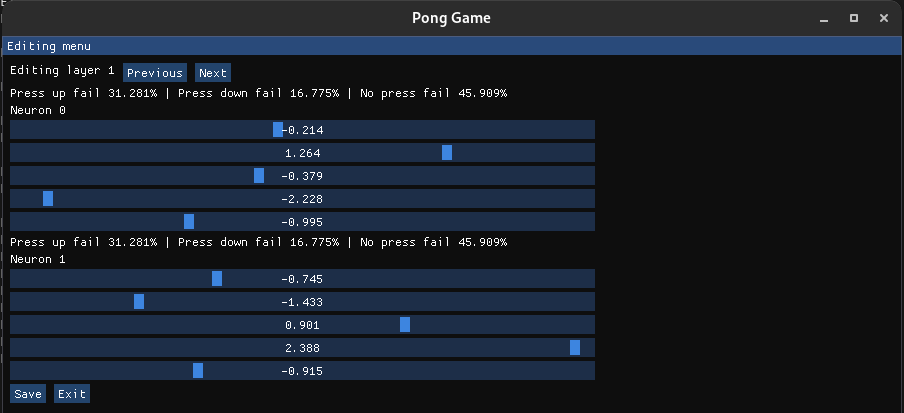
\includegraphics[width=15cm]{archivos/imagenes/menu-editar-pesos-red.png}
	\caption{Menú para editar pesos de la red neuronal.}
	\label{editar red neuronal}
\end{figure}
